
\begin{figure}[t]
\begin{center}
  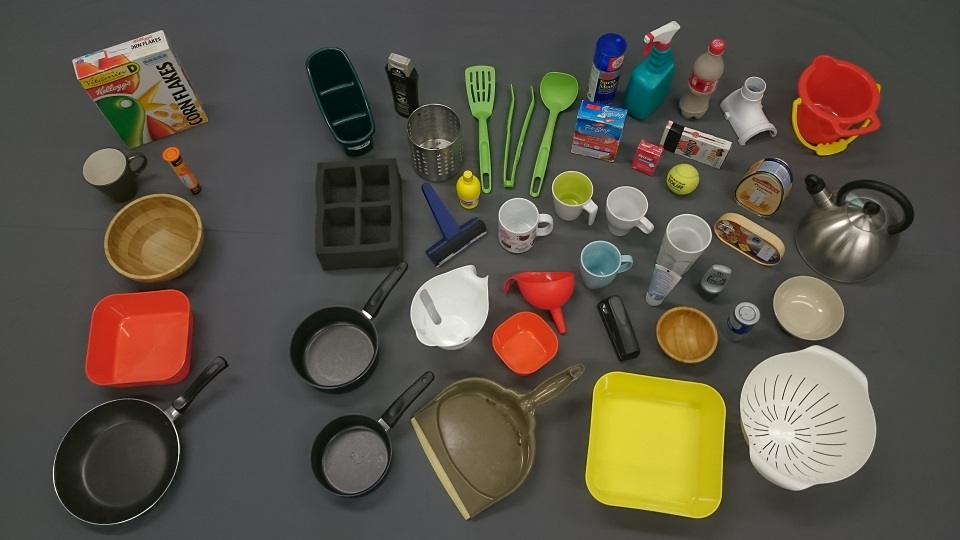
\includegraphics[width=0.9\linewidth]{images/objects.jpg}
  \end{center}
  \caption{The real objects. The training objects are on the left, testing objects are on the right.}
  \label{fig:real-objects}
\end{figure}

\begin{table}[b]
\begin{center}
\caption{Performance on the real robot \label{tab:robot-results}}
\begin{tabular}{|c|c|c|c|c|c|} \hline
Alg & \# succ & \% succ & Alg & \# succ & \% succ \\ \hline
V1  &  28 & 57.1\% & V4   & 37  & 75.5\% \\
V2  & 40 & 81.6\% & V11 & 43  & 87.8\% \\
\hline
\end{tabular}
\end{center}
\end{table}


We compared four variants on the real robot: V1, V2, V4 and V11. V1 and V2 are the pure generative models. V4 is, in simulation, the equal best generative-evaluative method using GM1 as the generative model. It uses EM2 as the evaluative model. V11 is, in simulation, the best performing generative-evaluative method using GM2 as the generative model. This selection allows us to compare the best generative-evaluative methods with their counterpart pure generative models. 

We employed the same real objects as described in \cite{kopicki2019ijrr}. This used 40 novel test objects (Figure~\ref{fig:real-objects}). Object-pose combinations were chosen to reduce the typical surface recovery. Some objects were employed in several poses, yielding 49 object-pose pairs. From the 40 objects, 35 belonged to object classes in the simulation dataset, while the remaining five did not. 

Using this data-set, all algorithms were evaluated on the real-robot using a paired trials methodology. Each was presented with the same object-pose combinations. Each variant generated a ranked list of grasps, and the highest ranked grasp was executed. The highest-ranked grasp based on the predicted success probability of an evaluative network is performed on each scene. A grasp was deemed successful if, when lifted for five seconds, the object then remained stable in the hand for a further five seconds. 

The results are shown in Table~\ref{tab:robot-results}. In each case, the GEA variant outperforms the equivalent pure GM variant. So that V4 outperforms V1 by 75.5\% grasp success rate to 57.1\% and V11 outperforms V2 87.8\% to 81.6\%. Thus, we have strong support for our main hypothesis, which is that a Generative-Evaluative architecture outperforms a pure generative model.
%The success rate for GM1 was 57.1\% and for the top-performing method based on GM1, GEA.1, it was 77.6\% (Table~\ref{tab:robot-results}). The success rate of the second baseline, GM2, is 81.6\%, while GEA.3 shows outperforms it with a success rate of 87.8\%. A two-tailed McNemar test, for the difference between success rates for paired comparison data, was performed. The difference between the two algorithms has a $p$-value of 0.0442, and so is statistically significant. A selection of grasps where the two methods performed differently are shown in Figure~\ref{fig:successfail}.

% OLD TABLE
%\begin{table}
%\begin{center}
%\caption{Results of the real robot paired comparison trial.}
%\begin{tabular}{|c|c|c|c|}  \hline 
%          &                & \multicolumn{2}{ c |}{ GM} \\ \hline
%          &                & \# succs & \# fails  \\  \hline
 %GEA  & \# succs &  23 &  15  \\
 %         & \# fails    &  5   &   6   \\ \hline
%\end{tabular}
%\end{center}
%\label{tab:robot-results}
%\end{table}

%\begin{table}
%\begin{center}
%\caption{Results of the real robot paired comparison trial.}
%\label{my-label}
%\begin{tabular}{|cc|c|c|l}
%\cline{1-4}
%                                           &         & \multicolumn{2}{c|}{GM} &  \\ \cline{3-4}
%                                           &         & \# succs    & \# fails    &  \\ \cline{1-4}
%\multicolumn{1}{|c|}{\multirow{2}{*}{GEA}} & \# succs & 23         & 15         &  \\
%\multicolumn{1}{|c|}{}                     & \# fails & 5          & 6          &  \\ \cline{1-4}
%\end{tabular}
%\end{center}
%\label{tab:robot-results}
%\end{table}

\begin{figure*}
\begin{center}
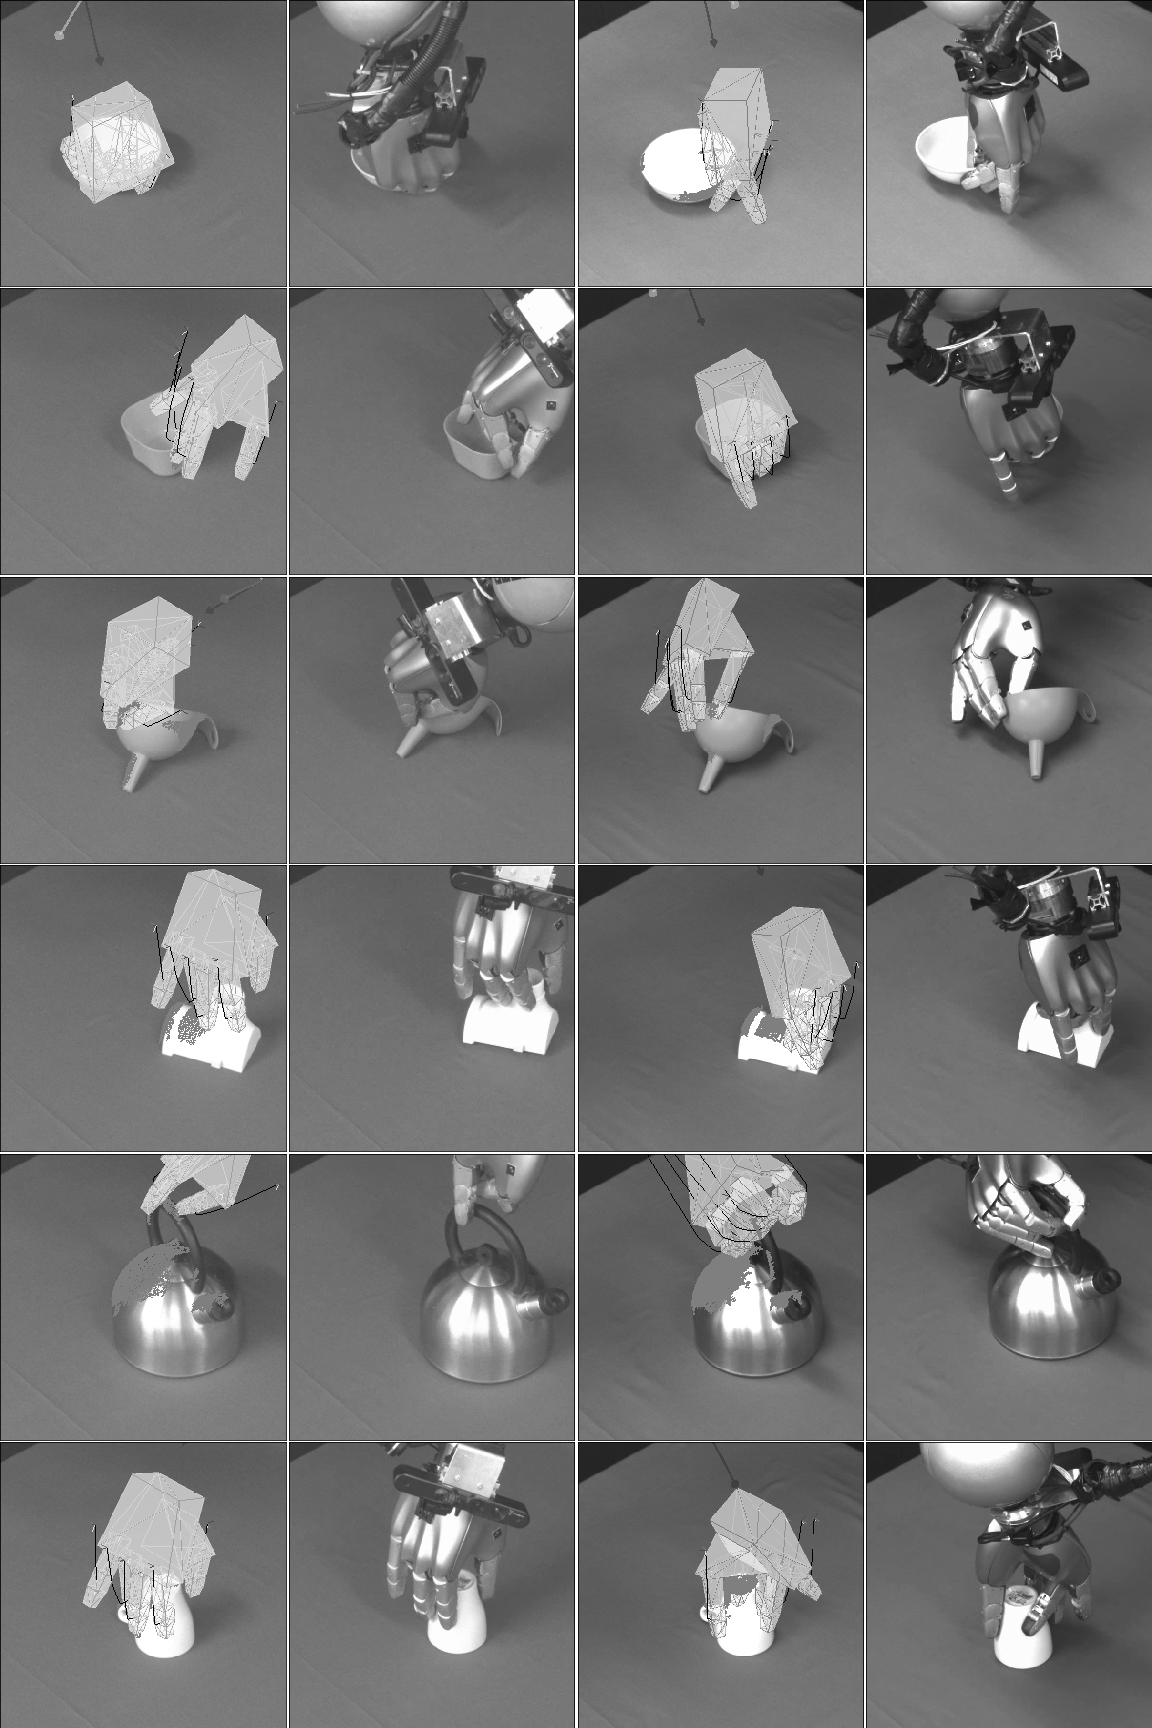
\includegraphics[width=0.5\textwidth]{plots/A2fA9s_1_vertical.png}~
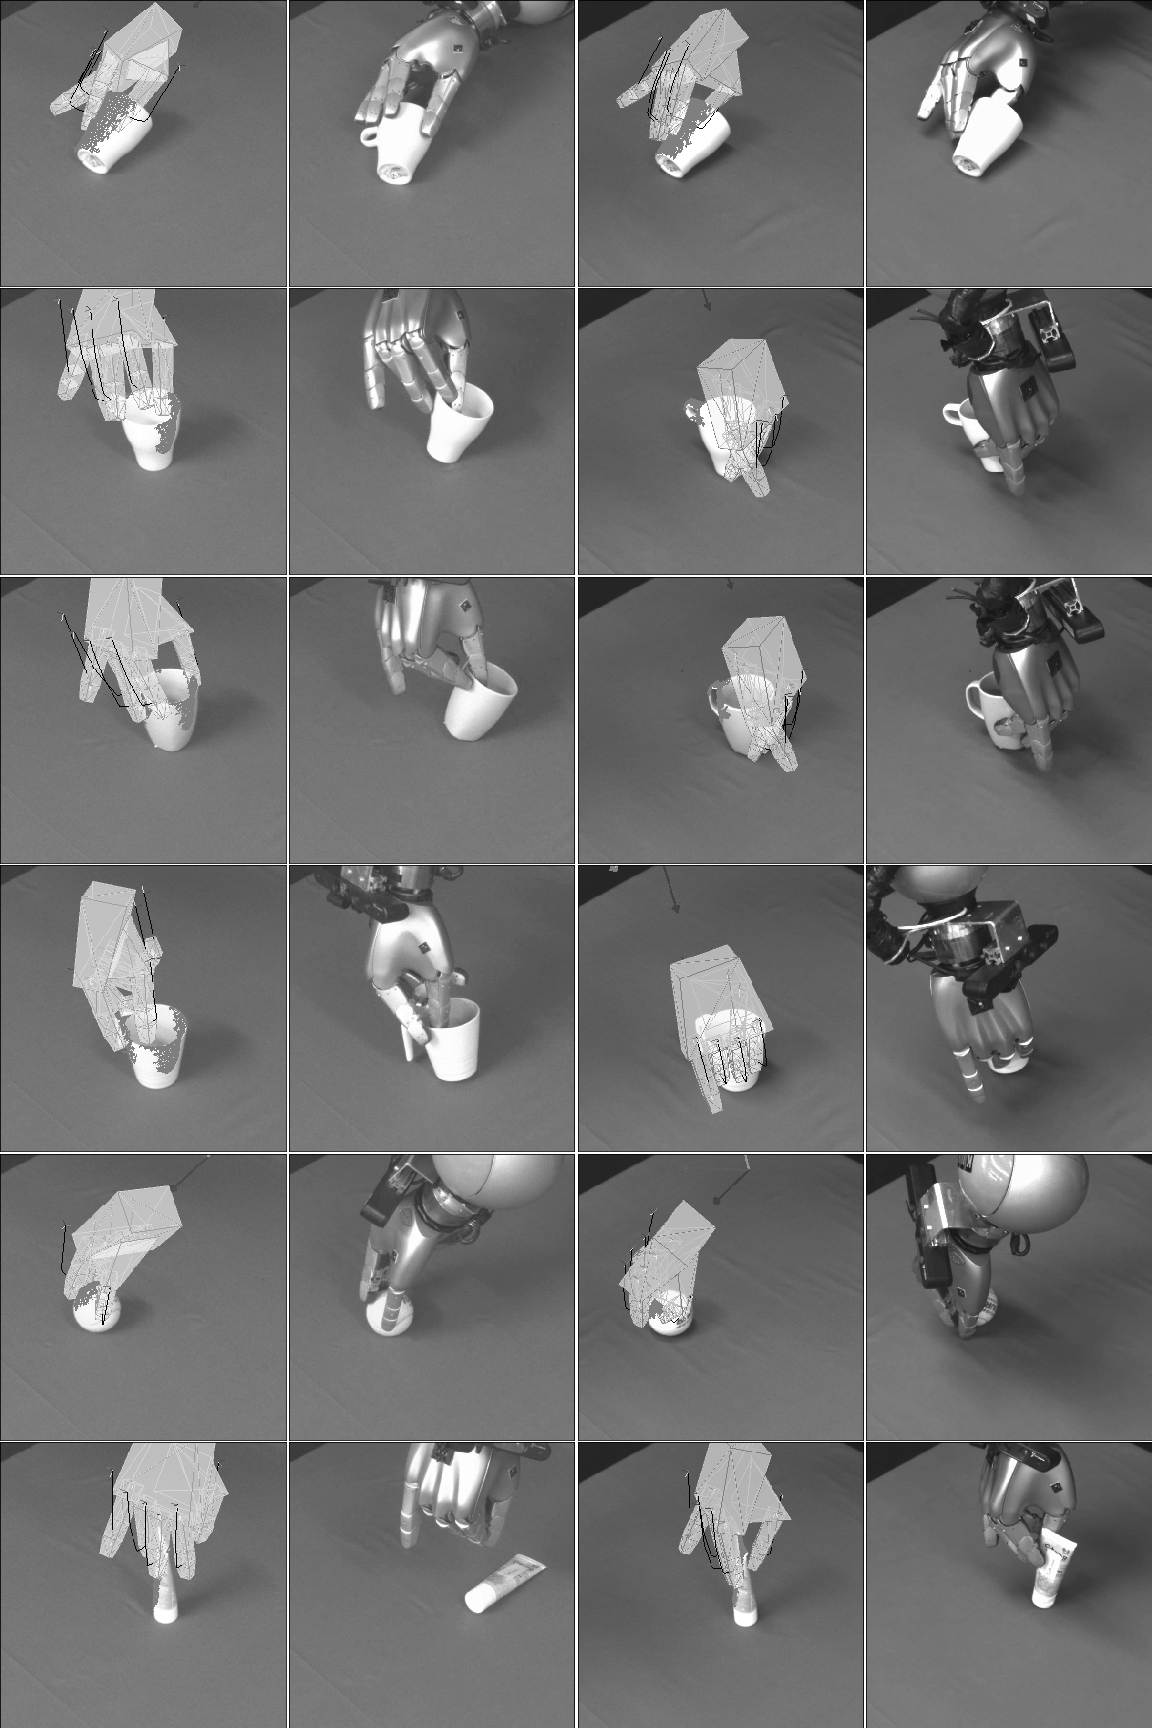
\includegraphics[width=0.5\textwidth]{plots/A2fA9s_2_vertical.png}
\caption{V1 vs V4. This shows grasps from methods based on generative model GM1. The V1 grasps are shown in columns 1-2 and 5-6. The corresponding V4 grasps are shown in columns 3-4 and 7-8. This figure shows the cases where V1 failed and V4 succeeded.\label{fig:v1fv4s}}
\end{center}
\end{figure*}


\begin{figure*}
\begin{center}
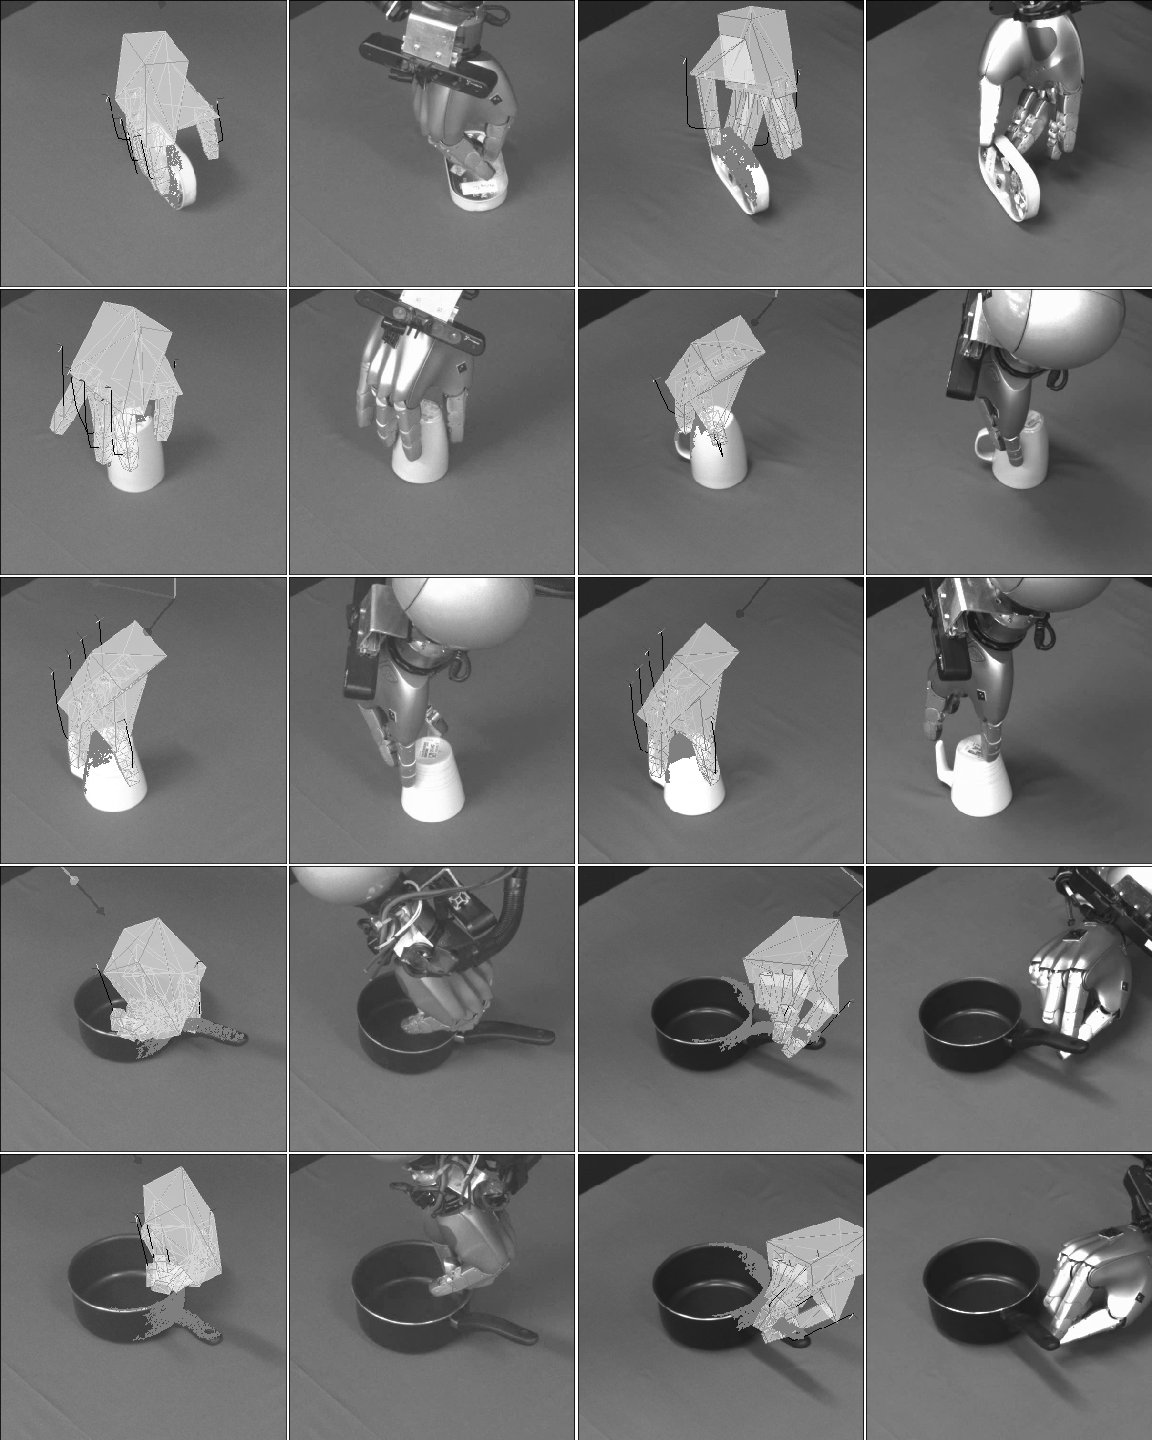
\includegraphics[width=0.5\textwidth]{plots/A2fA9f_vertical.png}~
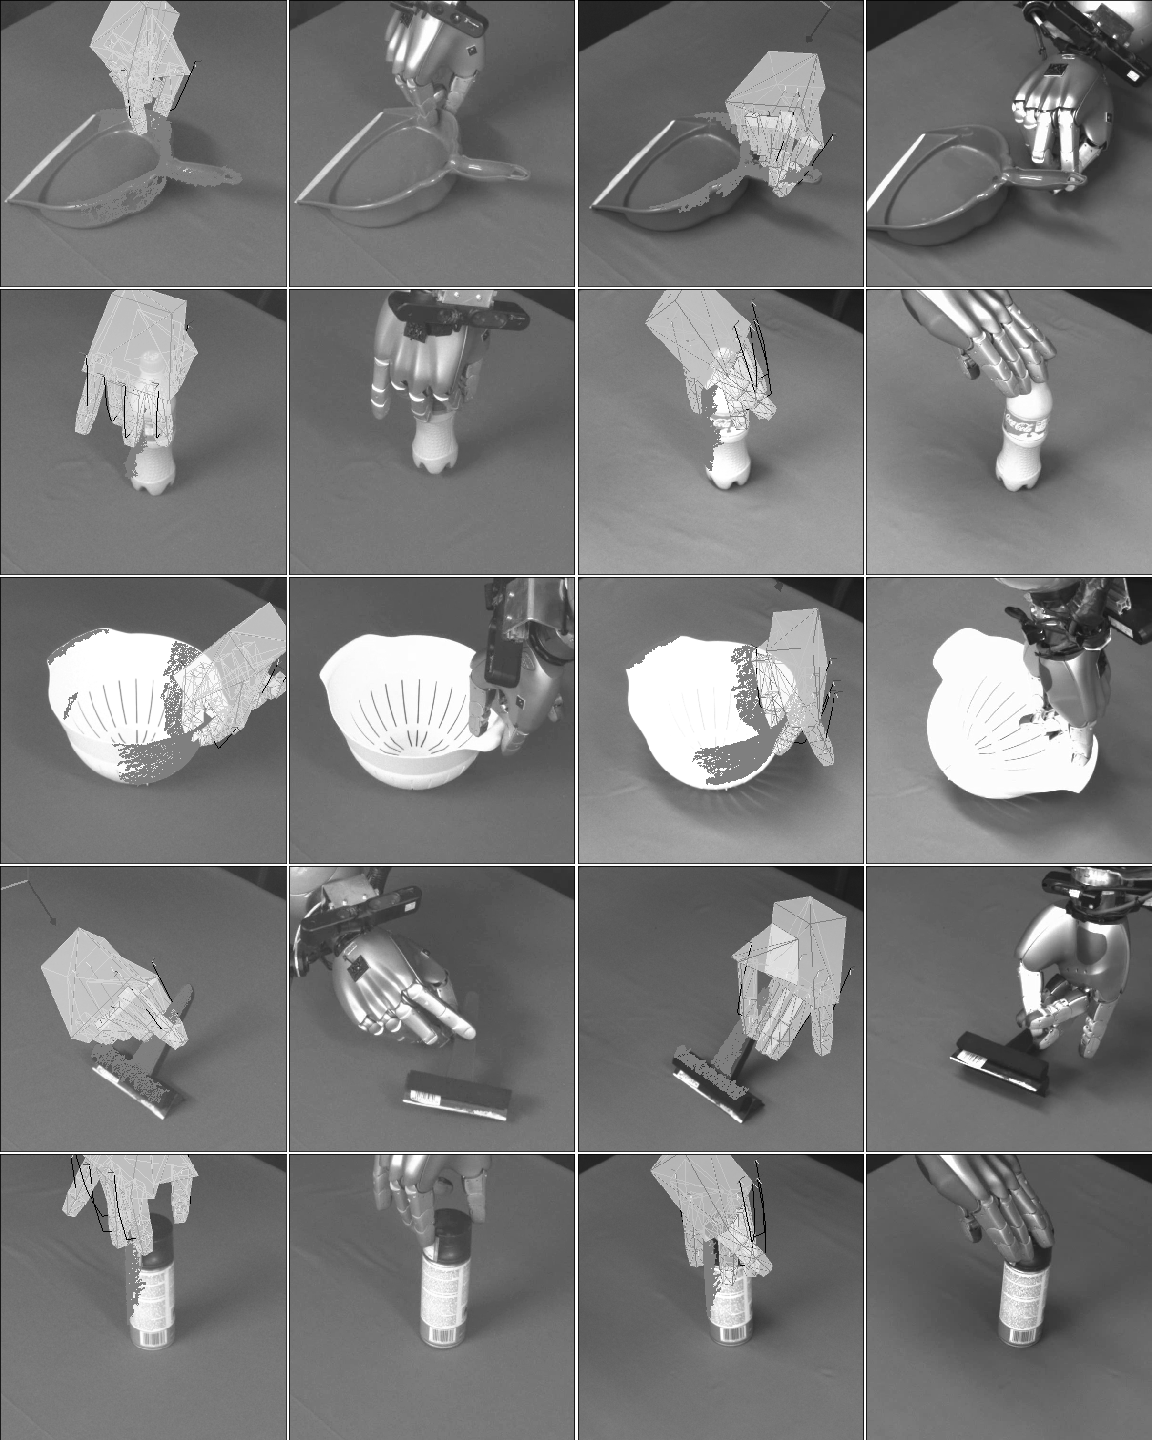
\includegraphics[width=0.5\textwidth]{plots/A2sA9f_vertical.png}
\caption{V1 vs V4. This shows grasps from methods based on generative model GM1. The V1 grasps are shown in columns 1-2 and 5-6. The corresponding V4 grasps are shown in columns 3-4 and 7-8. The left hand panel shows the cases where both V1 and V4 failed. The right hand panel shows the cases where V1 succeeded and V4 failed. \label{fig:v1fsv4f}}
\end{center}
\end{figure*}

\begin{figure}
\begin{center}
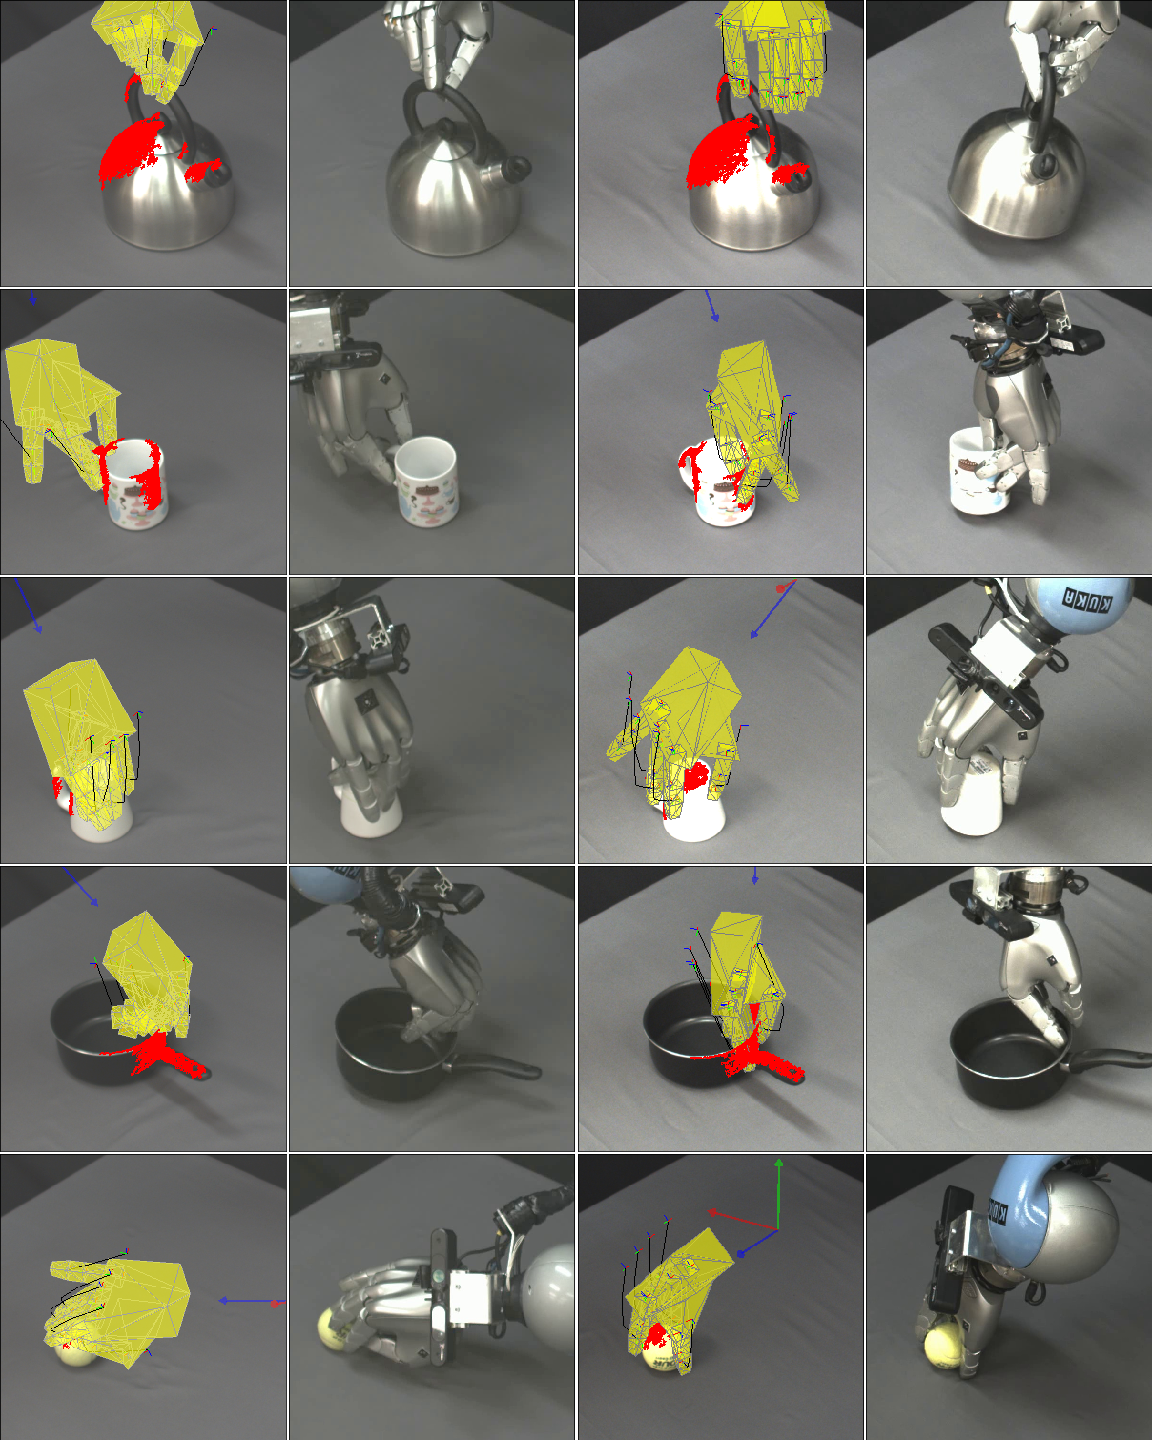
\includegraphics[width=\columnwidth]{plots/A6fA10s_vertical.png}
\caption{V2 vs V11. This shows grasps from methods based on generative model GM2. The V2 grasps are shown in columns 1-2. The corresponding V11 grasps are shown in columns 3-4. This figure shows the cases where V2 failed and V11 succeeded. \label{fig:v2fv11s}}
\end{center}
\end{figure}

\begin{figure}
\begin{center}
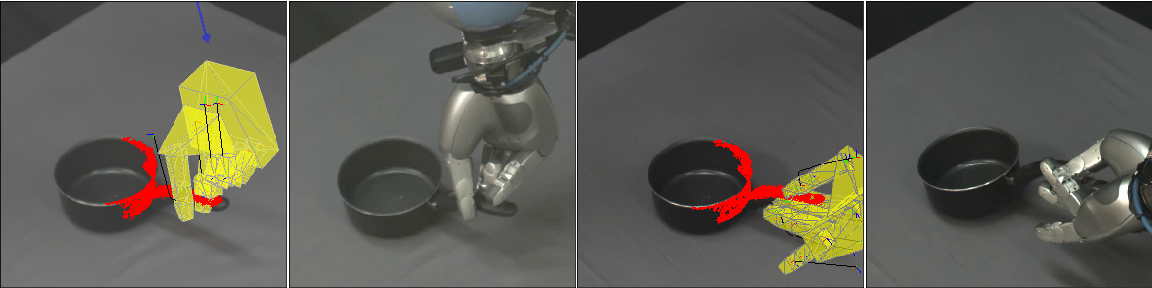
\includegraphics[width=\columnwidth]{plots/A6fA10f_vertical.png}\\
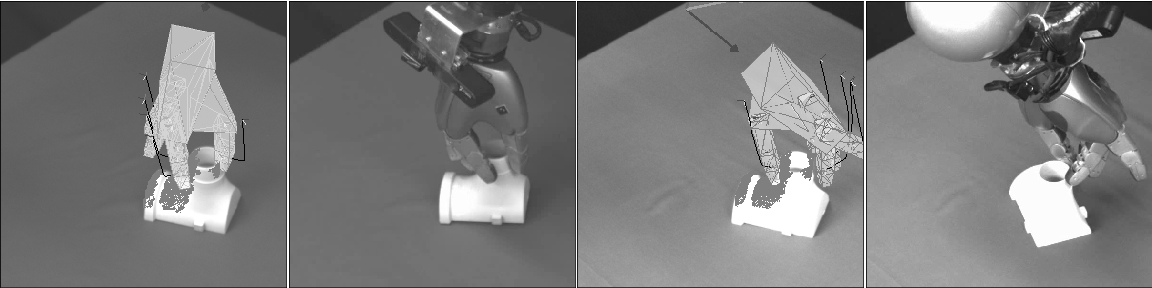
\includegraphics[width=\columnwidth]{plots/A6sA10f_vertical.png}
\caption{V2 vs V11. This shows grasps from methods based on generative model GM2. The V2 grasps are shown in columns 1-2. The corresponding V11 grasps are shown in columns 3-4. The top row shows the case where both V2 and V11 failed. The bottom row shows the case where V2 succeeded and V11 failed. \label{fig:v2fsv11f}}
\end{center}
\end{figure}

%\begin{figure*}
%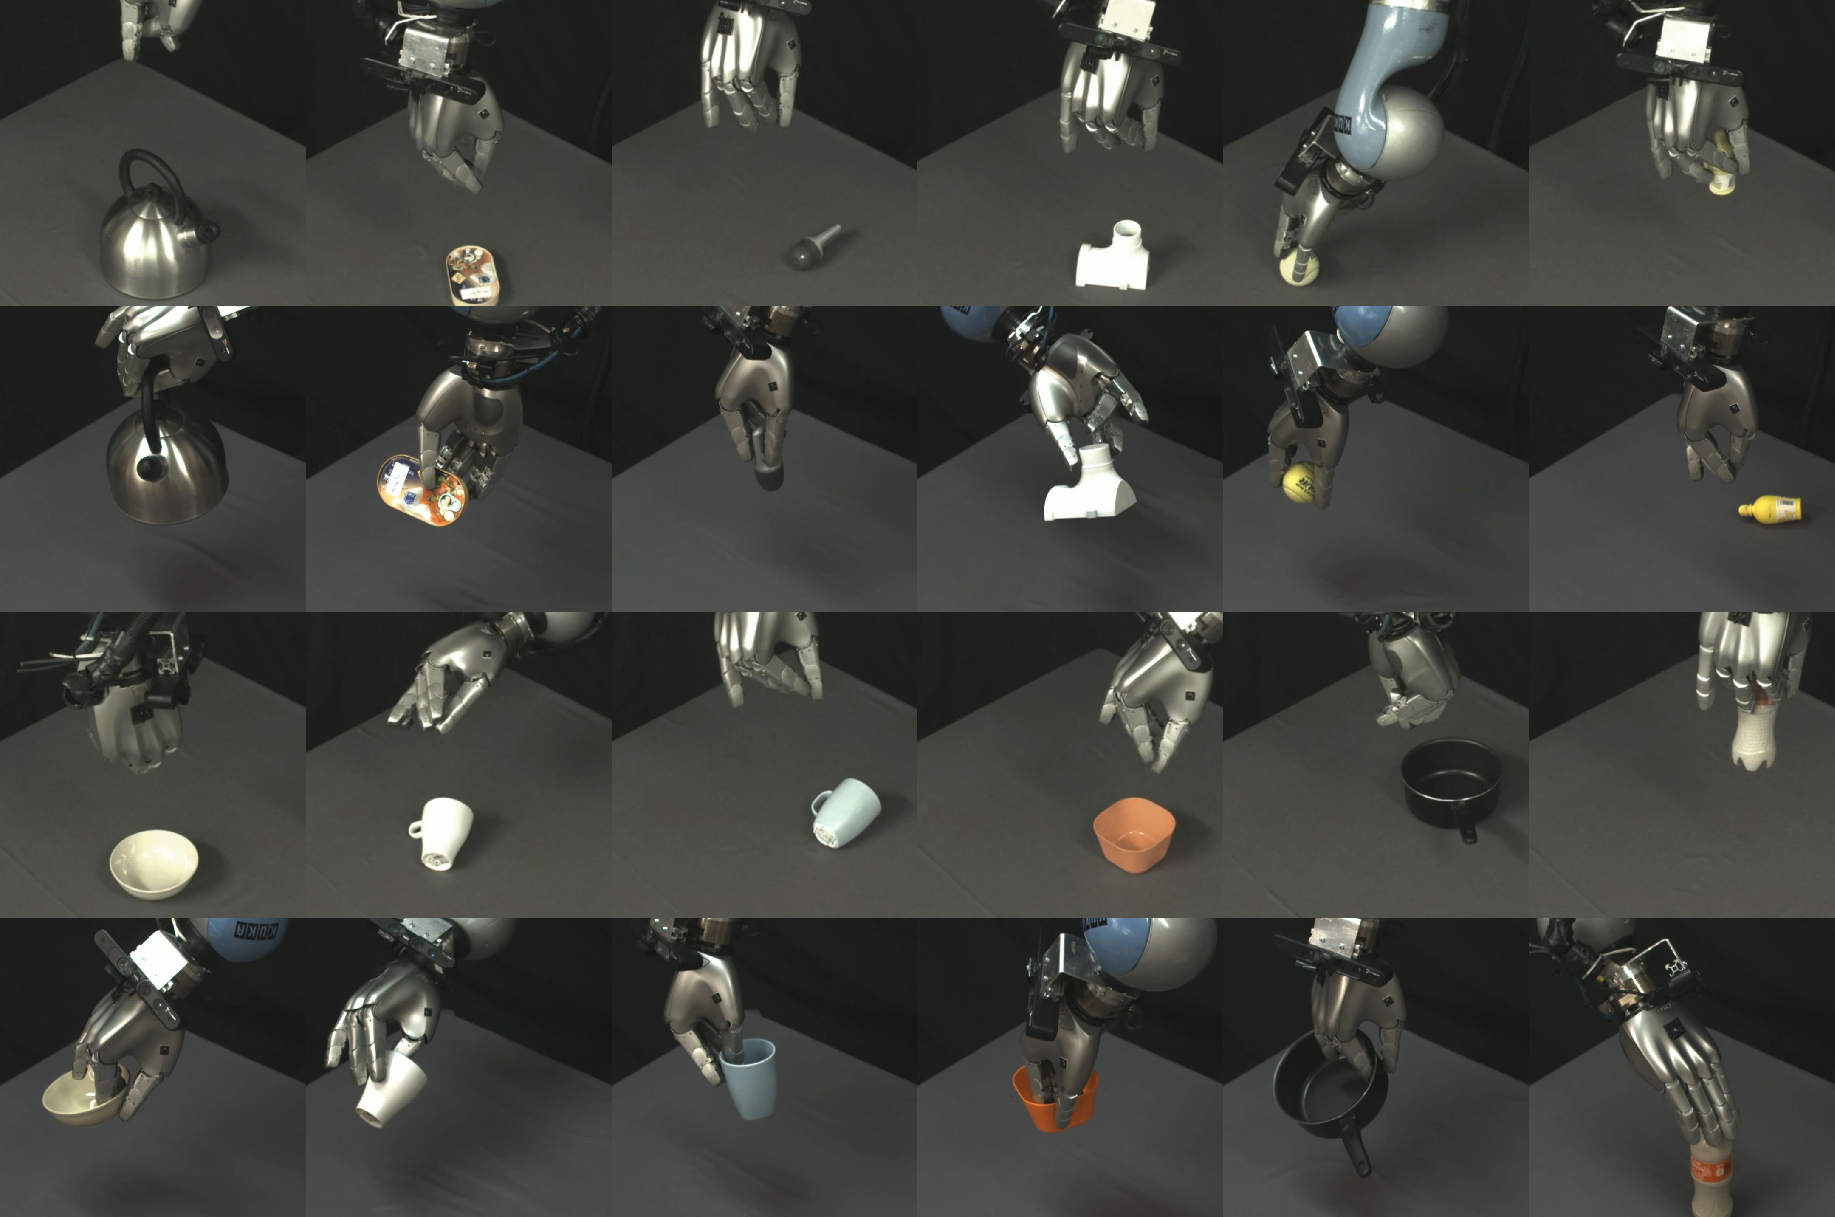
\includegraphics[width=\textwidth]{images/successfailure.pdf}
%\caption{Examples of grasps generated by the generative model (GM, $1^{st}$ and $3^{rd}$ row) and the generative-evaluative model (GEA, $2^{nd}$ and $4^{th}$ row) on paired trials. The first five columns show some of the 15 cases where the GEA model succeeds but GM fails. The far right-hand column shows 2 of the 5 converse cases. \label{fig:successfail}}
%\end{figure*}

%Training parameters for network. Training of example grasps for learning from demonstration. Creation of real test data set. Paired comparisons methodology with vanilla LFD algorithm (pose + object + camera view).
%
%The actual grasping tests have been performed on the real robot. 